\documentclass{beamer}
\usetheme{Boadilla}
\usepackage{essay-def}
\usepackage{bm}
\usepackage{amsfonts}
\usepackage{amssymb}
\usepackage{comment}
\usepackage{geometry}
\geometry{left=1cm,right=1cm}
\title{Wasserstein information matrix}
\author{Jiaxi Zhao (PKU)}
\institute[]{joint work with Wuchen Li (UCLA)}
\date{June 2020}
\begin{document}
\begin{frame}
\titlepage
\end{frame}

\begin{frame}{Distances on probability space}
    \begin{figure}[H]
          \centering
          \centerline{\includegraphics[width=0.6\linewidth]{history.png}}
  %        \caption{History of statistics and geometry}
        \end{figure}
\end{frame}

\begin{frame}{Information matrix}
Information matrix (a.k.a Fisher information matrix, Fisher-Rao metric) plays important roles in information science, statistics and machine learning:

\vspace{0.5cm}
\begin{itemize} 
\item 1. Population Games via Replicator Dynamics (Shahshahani, Smith);
%\item Reinforcement learning (Sutton and Barto; Alpha Go; Montufar);
%\item Numerics for gradient or Hamiltonian type PDEs;
\item 2. Machine learning: Natural gradient (Amari); ADAM (Kingma 2014); Stochastic relaxation (Malago) and many more in book {\em Information geometry} (Ay et.al.).
\item 3. \textbf{Statistics}: Kullback--Leibler (KL) divergence $\leftrightarrow$ Likelihood principle, Fisher information matrix $\leftrightarrow$ Cramer-Rao bound, 
\end{itemize}
\end{frame}

\begin{frame}{Learning}
Given a data measure $\rho_{\textrm{data}}(x)=\frac{1}{N}\sum_{i=1}^N\delta_{X_i}(x)$ and a parameterized model $\rho(x; \theta)$. 
%%Consider the following learning problem %(Eulerian)
Machine learning problems often refer to
\begin{equation*}
\begin{split}
\min_{\rho_\theta\in \rho(\Theta)}\quad D(\rho_{\textrm{data}}, \rho_\theta).
\end{split}
\end{equation*}
One typical choice of $D$ is the Kullback--Leibler divergence (relative entropy) $$D(\rho_{\textrm{data}}, \rho_\theta)=\int_{\Omega}\rho_{\textrm{data}}(x)\log\frac{\rho_{\textrm{data}}(x)}{\rho(x;\theta)}dx.$$
\end{frame}

\begin{frame}{Natural gradient}
The natural gradient method refers to
\begin{equation*}
\theta^{k+1}=\theta^k- h {\color{blue}G_F(\theta^k)^{-1}}\nabla_\theta D(\rho_{\textrm{data}}, \rho_{\theta^k}),
\end{equation*}
where $h>0$ is a stepsize and 
\begin{equation*}
\begin{split}
G_F(\theta)=&\mathbb{E}_{X\sim\rho_\theta}(\nabla_\theta \log\rho(X;\theta))^T(\nabla_\theta\log\rho(X;\theta)) 
\end{split}
\end{equation*}
 is the Fisher information matrix and $\nabla_\theta \log\rho(X;\theta)$ is named score function.

\begin{block}{Why natural gradient and Fisher information matrix?}
\begin{itemize}
\item {1. Parameterization invariant};
\item 2. Pre-conditioners for KL divergence related learning problems;  
\item {\color{red}3. Online Cramer-Rao bound}.
\end{itemize}
\end{block}
%\end{frame}
%In optimization, $G_F(\theta)$ is the Newton's method for KL divergence (relative entropy). 
\end{frame}
%%%
%%%

\begin{frame}{Optimal transport}
In recent years, optimal transport (a.k.a Earth mover's distance, Monge-Kantorovich problem, Wasserstein metric) has witnessed a lot of applications: %in probability related problems:
\vspace{0.5cm}
\begin{itemize} 
%%\item Image retrieval (Rubner 2000); Image segmentation (Chan 2006) etc;
%%\item Bakery Emery Calculus and Ricci curvature lower bound (Li 2018);
\item 1. Population Games via Fokker-Planck Equations (Degond et. al. 2014, Li et.al. 2016);
%\item Mean field games (Larsy, Lions, Gangbo);
\item 2. Machine learning: Wasserstein Training of Boltzmann Machines (Cuturi et.al. 2015); Learning from Wasserstein Loss (Frogner et.al. 2015); Wasserstein GAN (Bottou et.al. 2017); Wasserstein statistics, and many more in NIPS 2015, 2016, 2017, 2018, 2019.
\end{itemize}
\end{frame}

\begin{frame}{Why optimal transport?}
Optimal transport provides a particular distance ($W$) among histograms, which relies on the distance on sample spaces ({\color{blue}ground cost} $c$). 
\bequn
		\begin{aligned}
			W_c\lp \rho, \mu \rp & = \inf_{\pi \in \prod\lp \rho, \mu \rp} \int c\lp x, y \rp d\pi\lp x, y \rp,		\\
			W_p^p\lp \rho, \mu \rp & = \inf_{\pi \in \prod\lp \rho, \mu \rp} \int \lv x - y \rv^p d\pi\lp x, y \rp \ \text{(Wasserstein-p distance)}.
		\end{aligned}
	\eequn
Denote $X_0\sim \rho_0=\delta_{x_0}$, $X_1\sim \rho_1=\delta_{x_1}$. Compare
$$W(\rho_0,\rho_1)=\inf_{\pi\in\Pi(\rho_0, \rho_1)}\mathbb{E}_{(X_0, X_1)\sim\pi} c(X_0, X_1)=c(x_0,x_1);$$
Vs
$$\textrm{TV}(\rho_0,\rho_1)=\int_{\Omega}|\rho_0(x)-\rho_1(x)|dx=2;$$
Vs 
$$\textrm{KL}(\rho_0\|\rho_1)=\int_\Omega\rho_0(x)\log\frac{\rho_0(x)}{\rho_1(x)}dx=\infty.$$
\end{frame}


\begin{frame}{Wasserstein Loss function}
Given a data distribution $\rho_0$ and a probability model $\rho_{\theta}$. Consider
\begin{equation*}
\min_{\theta\in \Theta}~W(\rho_0, \rho_{\theta}).
\end{equation*}
This is a double minimization problem, i.e. 
\begin{equation*}
\begin{split}
&W(\rho_0, \rho_{\theta})
=\min_{\pi\in\Pi(\rho_0, \rho_{\theta})}\mathbb{E}_{(X_0, X_1)\sim\pi} c(X_0, X_1).
\end{split}
\end{equation*}
Many applications, such as Wasserstein GAN, Wasserstein Loss, are built on the above formulation.
\end{frame}



\begin{frame}{Goals}
\vspace{0cm}
\begin{block}{Main Question:}
Instead of looking at the Wasserstein metric, we propose the optimal transport induced \textbf{information matrix in probability models}, and study its properties on statistics and machine learning problems.
\end{block}

\begin{block}{Related studies}
\begin{itemize} 
\item 1. Wasserstein covariance (Petersen, Muller.)
\item 2. Wasserstein minimal distance estimator (Bernton, Jacob, Gerber, and Robert.)
\item 3. Wasserstein natural gradient (Li, Montufar, Chen, Lin, Abel et.al.)
\item 4. Statistical inference for generative models with maximum mean discrepancy (Briol, Barp, Duncan, Girolami.)
\end{itemize}
\end{block}
\end{frame}
\begin{frame}{Problem formulation}
%The optimal transport problem first introduced by Monge in 1781, relaxed by Kantorovich by 1940. It has three formulations under various angles:
\begin{itemize}
\item 1. Mapping formulation: Monge problem (1781): Monge-Amp{\' e}re equation\ ;
\item 2. Statical formulation:  Kantorovich problem (1940): Linear programming\ ;
\item 3. Dynamical formulation: {\color{blue}Density optimal control} (Nelson, Lafferty, Otto, Villani).
\end{itemize}
In this talk, we will apply {\color{blue}density optimal control} into learning problems.
\end{frame}

\begin{frame}{Density manifold}
Optimal transport has an optimal control reformulation by the dual of dual of linear programming:
\begin{equation*}
\inf_{\rho_t}~\int_0^1g_W(\partial_t\rho_t, \partial_t\rho_t)dt=\int_0^1\int_{\Omega}(\nabla\Phi_t, \nabla\Phi_t)\rho_tdxdt,
\end{equation*}
%%where the infimum runs over all vector fields $v_t=\nabla\Phi_t$, 
under the dynamical constraint, i.e. continuity equation: %{\color{red}continuity equation} holds     
\begin{equation*}
\partial_t\rho_t+\nabla\cdot(\rho_t \nabla\Phi_t)=0,\quad \rho_0=\rho^0,\quad \rho_1=\rho^1.
\end{equation*}
Here, $(\mathcal{P}(\Omega), g_W)$ forms an infinite-dimensional {\color{blue}Riemannian manifold}\footnote{John D. Lafferty: The density manifold and configuration space quantization, 1988.}. 
%\vspace{2cm}
\begin{figure}
%\begin{tabular}{ccc}
%t = 0 & t = 1/5 & t = 2/5 \\
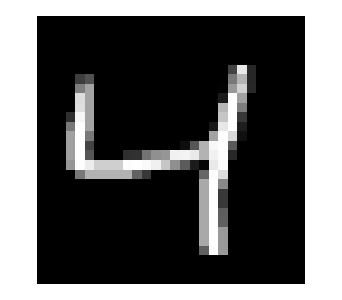
\includegraphics[width=.15\textwidth]{mnist_M1.eps} 
\includegraphics[width=.15\textwidth]{mnist_M2.eps} 
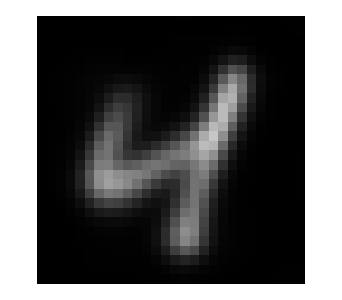
\includegraphics[width=.15\textwidth]{mnist_M3.eps}
%t = 3/5 & t = 4/5 & t = 1 \\
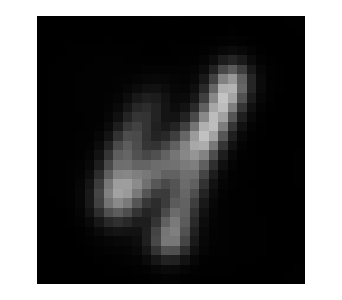
\includegraphics[width=.15\textwidth]{mnist_M4.eps} 
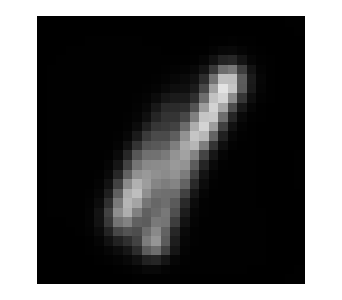
\includegraphics[width=.15\textwidth]{mnist_M5.eps} 
\includegraphics[width=.15\textwidth]{mnist_M6.eps} 
\end{figure}
\end{frame}

\begin{frame}{Information matrix}
    In parametric statistics, we study the finite dimensional statistical models parametrized by several parameters. Thus we need to establish a metric (information matrix) on these spaces.
    \begin{figure}[H]
          \centering
          \centerline{\includegraphics[width=0.5\linewidth]{pull_back.png}}
          \caption{Pull-back of the metric}
    \end{figure}
\end{frame}




\begin{frame}{Statistical information matrix}

    \begin{definition}[Statistical Information Matrix]
	Consider the density manifold $(\mathcal{P}(\mcX), g)$ with a metric tensor $g$, and a smoothly parametrized statistical model $ p_\theta$ with parameter $\theta\in\Theta \subset \mathbb{R}^d$. 
	Then the pull-back $G$ of $g$ onto the parameter space $\Theta$ is given by
	\begin{equation*}
	G(\theta)=\Big\langle \nabla_\theta p_\theta, g( p_\theta) \nabla_\theta p_\theta\Big\rangle.
	\end{equation*}
Denote $G(\theta)=(G(\theta)_{ij})_{1\leq i,j\leq d}$, then 
\begin{equation*}
G(\theta)_{ij}=\int_{\mathcal{X}}{\frac{\partial}{\partial \theta_i}p(x;\theta)\Big(g(p_\theta)\frac{\partial}{\partial \theta_j}p\Big)(x;\theta)}dx.
\end{equation*}
Here we name $g$ the statistical metric, and call $G$ the statistical information matrix.
\end{definition}
\end{frame}

\begin{frame}{Statistical information matrix}

    \begin{definition}[Score Function]
Denote $\Phi_i$ $\colon \mathcal{X}\times\Theta\rightarrow \mathbb{R}, i = 1,...,n $ satisfying
$$\Phi_i(x;\theta)= \lb g(p) \lp \frac{\partial}{\partial \theta_i}p(x;\theta) \rp \rb .$$
They are the score functions associated with the statistical information matrix $G$ and are equivalent classes in $C(\mathcal{X})/\mbR$. The representatives in the equivalent classes are determined by the following normalization condition:
\begin{equation*}\label{normalization}
    \mbE_{x \sim p_\theta} \Phi_i\lp x; \theta \rp = 0,\qquad i = 1,...,n.
\end{equation*}
Then the statistical metric tensor satisfies  
\begin{equation*}
G(\theta)_{ij}=\int_{\mathcal{X}} \Phi_i(x;\theta)\Big(g(p_\theta)^{-1}\Phi_j\Big)(x;\theta)dx.
\end{equation*}
\end{definition}
\end{frame}

\begin{frame}{Statistical information matrix}
    Formulating information matrices as expectations:
    \begin{itemize}
        \item Fisher Information Matrix
        \begin{equation*}
\begin{split}
G_F(\theta)_{ij}= \mathbb{E}_{p_\theta}\lp \frac{\partial}{\partial \theta_i}\log p(x;\theta)\frac{\partial}{\partial \theta_j}\log p(x;\theta) \rp.
\end{split}
\end{equation*}
        \item Wasserstein Information Matrix
        \begin{equation*}
\begin{split}
G_W(\theta)_{ij}=\ \mathbb{E}_{p_\theta}\lp \nabla_x\Phi_i^W(x;\theta), \nabla_x\Phi_j^W(x;\theta) \rp.
\end{split}
\end{equation*}
    \end{itemize}
\end{frame}

\begin{frame}{Poisson equation}
 %   \begin{proposition}[Poisson equation]\label{prop4}
The Wasserstein score functions $\Phi^W_i(x;\theta)$ satisfy the following Poisson equation
\begin{equation*}\label{ws}
\nabla_x \log p(x;\theta)\cdot \nabla_x\Phi^W_i(x;\theta)+\Delta_x\Phi^W_i(x;\theta)=-\frac{\partial}{\partial \theta_i}\log p(x;\theta).
\end{equation*}
%\end{proposition}
\end{frame}

\begin{frame}{Separability}
%    \begin{proposition}[Separability]\label{sep}
If $p(x;\theta)$ is an independence model, i.e. 
\begin{equation*}
    p(x,\theta) = \Pi_{k = 1}^n p_k(x_k;\theta),\quad x=(x_1,\cdots, x_n).
\end{equation*}
Then there exists a set of one dimensional functions $\Phi^{W,k}\colon \mathcal{X}_k \times\Theta_k\rightarrow \mathbb{R}$, such that 
\begin{equation*}\label{linear}
\Phi^W(x;\theta)=\sum_{k = 1}^n\Phi^{W,k}(x_k;\theta).
\end{equation*}
In addition, the Wasserstein information matrix is separable:
\begin{equation*}
G_W(\theta)=\sum_{k = 1}^nG_{W}^k(\theta),
\end{equation*}
where $G_{W}^k(\theta)=\mathbb{E}_{p_\theta} \lp \nabla_{x_k}\Phi^{W,k}(x;\theta), \nabla_{x_k}\Phi^{W,k}(x;\theta) \rp $.
%\end{proposition}
\end{frame}

\begin{frame}{One dimensional sample space}
%    \begin{proposition}[One dimensional sample space]
If $\mathcal{X}\subset \mathbb{R}^1$, the Wasserstein score functions satisfy
\begin{equation*}\label{1d}
\Phi_i^W(x;\theta)=-\int_{\mcX \cap \lb -\infty, x \rb} \frac{1}{p(z;\theta)}\frac{\partial}{\partial\theta_i}F(z;\theta)dz, 
\end{equation*}
 where $F(x;\theta)=\int p(y;\theta)dy$ is the cumulative distribution function. And the Wasserstein information matrix satisfies 
 \begin{equation*}
 G_W(\theta)_{ij}=\mathbb{E}_{p_\theta} \lp \frac{\frac{\partial}{\partial\theta_i}F(x;\theta)\frac{\partial}{\partial\theta_j}F(x;\theta)}{p(x;\theta)^2} \rp.
 \end{equation*}
% \end{proposition}
\end{frame}

\begin{frame}{Analytic examples of Wasserstein information matrix}
    Classical statistical models:
    \begin{itemize}
        \item Gaussian family:
        \begin{equation*}
            \begin{aligned}
                p(x;\mu,\sigma) & = \frac{1}{\sqrt{2\pi} \sigma}e^{-\frac{1}{2\sigma^2}(x-\mu)^2},            \\
                G_W(\mu,\sigma)& = \begin{pmatrix}
                1& 0 \\
                0 &  1
                \end{pmatrix}.
            \end{aligned}
        \end{equation*}
        \item Laplacian family:
        \begin{equation*}
            \begin{aligned}
                p(x;m,\lambda) & = \frac{\lambda}{2}e^{-\lambda|x-m|},            \\ G_W(\mu,\sigma)& = \begin{pmatrix}
                1& 0 \\
                0 &  \frac{2}{\lambda^4}
                \end{pmatrix}.
            \end{aligned}
        \end{equation*}
    \end{itemize}
\end{frame}

\begin{frame}{Analytic examples of Wasserstein information matrix}
    Generative models:
    \begin{itemize}
        \item Continuous 1-d generative family:
        \begin{equation*}
            \begin{aligned}
                p(\cdot;\theta) & = f_{\theta *}p_0\lp \cdot \rp,\ p_0 \text{ a given distribution,}            \\
                G_W(\theta) & = \int \lv \nabla_{\theta} f_{\theta}\lp x\rp \rv^2 p_0\lp x \rp dx,
            \end{aligned}
        \end{equation*}
        where the push-forward distribution is defined as
        \begin{equation*}
    \int_{A}p_0dx = \int_{f_{\theta }^{-1}(A)}f_{\theta *}p_0dx,
        \end{equation*}
    \end{itemize}
\end{frame}

\begin{frame}{Analytic examples of Wasserstein information matrix}
    Generative models with ReLU family:
        \begin{equation*}
            \begin{aligned}
                f_{\theta} \lp x \rp & = \ \sigma\lp x - \theta \rp = \lbb
        		\begin{aligned}
        		& 0, \qquad \qquad x \leq \theta,			\\
        		& x - \theta, \ \qquad x > \theta.
        		\end{aligned}\right.      \\
                G_W(\theta) & = F_0(\theta), \ F_0 \text{ cumulative distribution function of } p_0.
            \end{aligned}
        \end{equation*}
      %  \item 
       % Can we use this to analysis the dynamics systems appeared in machine learning?
        \begin{figure}[H]
          \centering
          \centerline{\includegraphics[width=0.5\linewidth]{ReLU.jpg}}
          \caption{This figure plots two examples of the push-forward family with $\theta_1 = 3, \theta_2 = 5$.}
        \end{figure}
 %   \end{itemize}
\end{frame}

\begin{frame}{Statistical Information Matrix}
    \begin{table}[h]
\setlength{\belowcaptionskip}{-0.cm}
\setlength{\floatsep}{0cm}
%\hspace{-4.0cm}
\centering
    \resizebox{\textwidth}{0.25\textwidth}{
\begin{tabular}{|l|c|c|}
\hline 
Probability Family & Wasserstein information matrix & Fisher information matrix \\
\hline
$
\begin{aligned}
    & \text{Uniform:}        \\
    & p(x;a,b) = \frac{1}{b - a}\mathbf{1}_{(a,b)}(x)
\end{aligned} $
 & $G_W(a,b) = \frac{1}{3} \begin{pmatrix}
1 & \frac{1}{2}\\
\frac{1}{2} &  1
\end{pmatrix}$ & $G_F(a,b)$ not well-defined 
\\
\hline
$
\begin{aligned}
    & \text{Gaussian:}        \\
    & p(x;\mu,\sigma)=\frac{e^{-\frac{1}{2\sigma^2}(x-\mu)^2}}{\sqrt{2\pi} \sigma}
\end{aligned}$ & $G_W(\mu,\sigma)=\begin{pmatrix}
1& 0 \\
0 &  1
\end{pmatrix}$ &  $G_F(\mu,\sigma) = \begin{pmatrix}
			\frac{1}{\sigma^2} & 0		\\
			0 & \frac{2}{\sigma^2}
		\end{pmatrix}$    
\\
\hline
$
\begin{aligned}
    & \text{Exponential:}        \\
    & p(x;m,\lambda) = \lambda e^{-\lambda\lp x - m \rp}
\end{aligned}$
& $G_W(m,\lambda)=\begin{pmatrix}
    1 & \frac{1}{\lambda^2}     \\
    \frac{1}{\lambda^2} & \frac{2}{\lambda^4}
\end{pmatrix}$ & $G_F(m,\lambda)$ not well-defined 
\\    
\hline
$
\begin{aligned}
    & \text{Laplacian:}        \\
    & p(x;m,\lambda) = \frac{\lambda}{2}e^{-\lambda|x-m|}
\end{aligned}
 $ & $G_W(m,\lambda)=\begin{pmatrix}
    1 & 0     \\
    0 & \frac{2}{\lambda^4}
\end{pmatrix}$ & 
$G_F(m,\lambda) = \begin{pmatrix}
			\lambda^2 & 0		\\
			0 & \frac{1}{\lambda^2}
		\end{pmatrix}$ 
\\    
\hline
$\begin{aligned}
    & \text{Location-scale:}        \\
    & p(x;m,\lambda) = \frac{1}{\lambda}p(\frac{x - p}{\lambda})
\end{aligned}$ & $G_W(\lambda,m)=\begin{pmatrix}
    \frac{\mathbb{E}_{\lambda,m}x^2-2m\mathbb{E}_{\lambda,m}x+m^2}{\lambda^2} & 0     \\
    0 & 1
\end{pmatrix}$ & 
$G_F(\lambda,m) = \begin{pmatrix}
			\frac{1}{\lambda^2} \lp 1 + \int_{\mbR} \lp \frac{\lp x - m \rp^2 p'^2}{\lambda^2 p} + \frac{\lp x - m \rp p'}{\lambda}\rp dx  \rp & \int_{\mathbb{R}}  \frac{(x - m)p'^2}{\lambda^3p} dx		\\
			\int_{\mathbb{R}}  \frac{(x - m)p'^2}{\lambda^3p} dx & \frac{1}{\lambda^2}\int_{\mathbb{R}} \frac{p'^2}{p} dx
		\end{pmatrix}$ 
		\\    
\hline
$
\begin{aligned}
    & \text{Independent:}        \\
    & p(x,y;\theta) = p(x;\theta)p(y;\theta)
\end{aligned}
 $ & $G_W(x,y;\theta)=G_W^1(x;\theta)+G_W^2(y;\theta)$ &
$G_F(x,y;\theta)=G_F^1(x;\theta)+G_F^2(y;\theta)$    \\    
\hline
$
\begin{aligned}
    \text{ReLU} &\text{ push-forward:}        \\
    & p(x;\theta) = f_{\theta*}p(x), \\ f_{\theta} \ \theta&\text{-parameterized ReLUs.}.
\end{aligned}
 $ & $G_W \lp \theta \rp= F\lp \theta \rp$, $F$ cdf of $p(x)$ &
$G_F(\theta)$ not well-defined   \\    
\hline
\end{tabular}}
\label{table1}
\caption{In this table, we present Wasserstein, Fisher information matrices for various probability families.}
\end{table}
\end{frame}



%%%%%%%%%%%%%%%%%%%
\begin{comment}
\begin{frame}{Information matrices \& Kernel method}
	\par
    Information matrices have intrinsic connection with kernel method in machine learning. The following is several important and intensively studied kernel.
    \begin{itemize}
        \item 1. Fisher kernel
        \item 2. Graph kernel
        \item 3. Neural tangent kernel
    \end{itemize}   

\end{frame}


\begin{frame}{Fisher kernel}
	\par
    Given a statistical model $\Theta \rightarrow \mcP\lp \mcX \rp: \theta \mapsto p\lp x; \theta \rp$, the Fisher kernel is given by
    \bequn
    	\begin{aligned}
    		\Phi_x = \nabla_{\theta} \log p\lp x; \theta \rp,			\\
		K_{\theta}\lp x, y \rp = \Phi_x^T I\lp \theta \rp^{-1} \Phi_y,
	\end{aligned}
    \eequn
    where $I\lp \theta \rp$ is the Fisher information matrix. 
    \par
    An important equality is
    \bequn
    	\begin{aligned}
		\mbE_{p_{\theta}}\lb K_{\theta}\lp x, y \rp \Phi_y^T \rb = & \ \int_{\mcX} K_{\theta}\lp x, y \rp \Phi_y^T p\lp y; \theta \rp dy		\\
		= & \ \int_{\mcX} \Phi_x^T I\lp \theta \rp^{-1} \Phi_y \Phi_y^T p\lp y; \theta \rp dy		\\
		= & \ \Phi_x^T I\lp \theta \rp^{-1} \int_{\mcX}  \Phi_y \Phi_y^T p\lp y; \theta \rp dy		\\
		= & \ \Phi_x^T I\lp \theta \rp^{-1} I\lp \theta \rp		\\
		= & \ \Phi_x^T.
	\end{aligned}	
    \eequn
\end{frame}


\begin{frame}{How about Wasserstein kernel?}
	\par
    Previous definition and properties concerned with Fisher kernel generalized easily to Wasserstein and other metric on probability space such as MMD...
    	\par

	Interesting questions include
    \begin{itemize}
        \item 1. Wasserstein Kernel for specific models
        \item 2. Relation to Stein metric
        \item 3. Geometric analysis associated with kernelized version
    \end{itemize} 
\end{frame}


\end{comment}
%%%%%%%%%%%%%%%%%%


\begin{frame}{Classical (Fisher) statistics \& Wasserstein statistics}
    We develop a parallel Wasserstein statistics following the classical statistics approach
    \begin{itemize}
        \item 1. Covariance $\stackrel{\text{inner product}}{\longrightarrow}$ Wasserstein covariance
        \item 2. Cramer-Rao bound $\stackrel{\text{cotangent space}}{\longrightarrow}$ Wasserstein-Cramer-Rao bound
        \item 3. Natural gradient efficiency $\stackrel{\text{separability}}{\longrightarrow}$ Wasserstein Natural gradient efficiency
    \end{itemize}   

\end{frame}

\begin{frame}{Wasserstein covariance}

\begin{definition}[Wasserstein covariance]
Given a statistical model $\Theta$, denote the Wasserstein covariance as follows:
\begin{equation*}
\mathrm{Cov}^W_\theta[T_1, T_2]=\mathbb{E}_{p_\theta} \lp \nabla_x T_1(x), \nabla_x T_2(x)^{T} \rp,
\end{equation*}
where $T_1$, $T_2$ are random variables as functions of $x$ and the expectation is taken w.r.t. $x \sim p_\theta$. 
Denote the Wasserstein variance: 
\begin{equation*}
\mathrm{Var}^W_\theta[T] = \mathbb{E}_{p_\theta} \lp \nabla_x T(x), \nabla_x T(x)^{T} \rp.
\end{equation*}
\end{definition} 
\begin{problem}
How does the Wasserstein covariance describe the variance of an estimator for Wasserstein stochastic gradient descent?
\end{problem}
\end{frame}

\begin{frame}{Wasserstein-Cramer-Rao bound}
\begin{theorem}[Wasserstein-Cramer-Rao inequalities]\label{WCR}
Given any set of statistics $T = \left( T_1,...,T_n\right) \colon \mathcal{X}\rightarrow \mathbb{R}^n$, where $n$ is the number of the statistics, define two matrices $\mathrm{Cov}^W_\theta[T(x)]$, $ \nabla_\theta \mathbb{E}_{p_\theta} [T(x)]^{T}$ as below:
\begin{equation*}
    \mathrm{Cov}^W_\theta[T(x)]_{ij} = \mathrm{Cov}^W_\theta[T_i,T_j], \qquad \nabla_\theta \mathbb{E}_{p_\theta} [T(x)]^{T}_{ij} = \frac{\pa}{\pa \theta_j} \mathbb{E}_{p_\theta} [T_i(x)],
\end{equation*}
then
\begin{equation*}
\mathrm{Cov}^W_\theta[T(x)] \succeq \nabla_\theta \mathbb{E}_{p_\theta} [T(x)]^{T}G_W(\theta)^{-1}\nabla_\theta \mathbb{E}_{p_\theta} [T(x)]. 
\end{equation*}
\end{theorem}
\end{frame}

\begin{frame}{Cramer-Rao bound: Fisher vs Wasserstein}
    \begin{itemize}
        \item Gaussian:
        \begin{equation*}
            G_W(\mu,\sigma)=\begin{pmatrix}
1 & 0 \\
0 &  1
\end{pmatrix}, \ G_F(\mu,\sigma) = \begin{pmatrix}
			\frac{1}{\sigma^2} & 0		\\
			0 & \frac{2}{\sigma^2}
		\end{pmatrix}.
        \end{equation*}
        \item Exponential:
        \begin{equation*}
            G_W(m,\lambda)=\begin{pmatrix}
    1 & \frac{1}{\lambda^2}     \\
    \frac{1}{\lambda^2} & \frac{2}{\lambda^4}
\end{pmatrix}, \ G_F \text{ not well-defined}.
        \end{equation*}
        \item Comparison:
        $G_W$ is well-defined for wider range of families.
         \item Tighter bound on the variance of an estimator
    \end{itemize}

\end{frame}

%%%%%%%%%%%%%%
\begin{comment}


\begin{frame}{Functional inequalities}
Comparison between Fisher and Wasserstein information matrices relates to well-known functional inequalities. Here we study them in parameter statistics. 
\begin{itemize}
    \item Dissipation of entropy \& Fisher information functional
    \begin{equation*}
        \begin{aligned}
            \frac{d}{dt} H(\mu|\nu) &= - \int_{\mathcal{X}} \lv \nabla_x \log \frac{\mu(x)}{\nu(x)} \rv^2 \mu(x) dx =  - I(\mu|\nu)        \\
            \frac{d}{dt} H(\mu|\nu) &= - \nabla_{\theta} \wtd H^T \wtd G_W^{-1}\nabla_{\theta} \wtd H = - I(\mu|\nu)     
        \end{aligned}
    \end{equation*}
    \item
    Log-Sobolev inequality (LSI)
    \begin{equation*}
        \begin{aligned}
            H(\mu|\nu) & < \frac{1}{2\alpha}I(\mu|\nu), \qquad \mu \in \mathcal{P}(\mathcal{X})         \\
            \wtd H(p_\theta|p_{\theta_*}) & < \frac{1}{2\alpha}\wtd I(p_\theta|p_{\theta_*}), \qquad \theta \in \Theta  
        \end{aligned}
    \end{equation*}
\end{itemize}
\end{frame}



\begin{frame}{Functional inequalities via Wasserstein and Fisher information matrices}
    \begin{theorem}[RIW-condition\footnote{Li, Geometry of probability simplex via optimal transport, 2018.} \footnote{Li, Montufar, Ricci curvature for parameter statistics, 2018.}]\label{RIW}
    The information matrix criterion for LSI can be written as:
    \begin{equation*}
        G_F\lp \theta \rp +  \nabla_{\theta}^2p_\theta\log \frac{p_\theta}{p_{\theta_*}} - \Gamma^W \nabla_{\theta}\wtd H(p_\theta|p_{\theta_*}) \geq 2\alpha G_W(\theta),
    \end{equation*}
    where $\Gamma^W$ is the Christoffel symbol in Wasserstein statistical model $\Theta$, while for PI can be written as:
    \begin{equation*}
        G_F\lp \theta \rp +  \nabla_{\theta}^2p_\theta\log \frac{p_\theta}{p_{\theta_*}} \geq 2\alpha G_W(\theta).
    \end{equation*}
\end{theorem}
\end{frame}

\end{comment}
%%%%%%%%%%%%%%%%%%


\begin{frame}{Wasserstein natural gradient}
Given a Loss function $\mathcal{F}\colon \mathcal{P}(\Omega)\rightarrow \mathbb{R}$ and probability model $\rho(\cdot, \theta)$, the associated gradient flow on a Riemannian manifold is defined by 
\begin{equation*}
\frac{d\theta}{dt}=-\nabla_g\mathcal{F}(\rho(\cdot, \theta)).
\end{equation*}
Here $\nabla_g$ is the Riemannian gradient operator satisfying
\begin{equation*}
g_{\theta}(\nabla_g\mathcal{F}(\rho(\cdot, \theta)),\xi)=\nabla_\theta \mathcal{F}(\rho(\cdot, \theta))\cdot \xi
\end{equation*}
for any tangent vector $\xi\in T_\theta\Theta$, where $\nabla_\theta$ represents the w.r.t. $\theta$ (Euclidean gradient). 
\end{frame}
\begin{frame}{Wasserstein natural gradient}

\begin{block}

	The gradient flow of Loss function $\mathcal{F}(\rho(\cdot, \theta))$ in $(\Theta, g_{\theta})$ satisfies
	\begin{equation*}
	\label{eqn:gradient flow}
	\frac{d\theta}{dt}=-G_W(\theta)^{-1}\nabla_{\theta} \mathcal{F}(\rho(\cdot, \theta)).
	\end{equation*}
\end{block}

If $\rho(\cdot; \theta)=\rho(x)$ is an identity map, then we recover the Wasserstein gradient flow in full probability space:
\begin{equation*}
\partial_t\rho_t=\nabla\cdot(\rho_t\nabla \frac{\delta}{\delta\rho}\mathcal{F}(\rho_t)).
\end{equation*}
\end{frame}
%%%\begin{frame}{Wasserstein natural gradient}
%%%What is natural gradient?
%%%\par
%%%Natural gradient is the gradient associated with a specific metric structure, such as Fisher-Rao metric, Wasserstein metric.
%%%\begin{definition}[Wasserstein natural gradient]
%%%    Given a statistical model $\Theta$ and a function $f$ on it. The Wasserstein natural gradient is defined by
%%%    \begin{equation*}\label{iterate}
%%%	\nabla_{\theta}^W f(\theta) = G_W^{-1} \nabla f(\theta),
%%%    \end{equation*}
%%%    where $\nabla f(\theta)$ is original Euclidean gradient.
%%%\end{definition}
%%%\end{frame}

\begin{frame}{Online natural gradient algorithm}
    We sample from the unknown distribution once in each step, and use sample $x_t$ to get new estimator $\theta_{t + 1}$
    \begin{equation*}\label{iterate}
	\theta_{t+1} = \theta_t -\frac{1}{t}\nabla_{\theta}^W l(x_t, \theta_t).
\end{equation*}
In order to analysis the convergence of this online algorithm, we define the Wasserstein covariance matrix $V_t$ to be
\begin{equation*}
    V_{t} = \mbE_{p_{\theta_*}}\lb \nabla (\theta_t - \theta_* ) \cdot \nabla (\theta_t - \theta_* )^T \rb,
\end{equation*}
where $\theta_*$ is the optimal value.
\begin{definition}[Natural gradient efficiency]
    The Wasserstein natural gradient is asymptotic efficient if
    \begin{equation*}
        V_t = \frac{1}{t}G_W^{-1}\lp \theta_* \rp + O(\frac{1}{t^2}).
    \end{equation*}
\end{definition}
\end{frame}

\begin{frame}{Covariance update}
\begin{theorem}[Variance updating equation of the Wasserstein Natural Gradient]\label{update}
For any function $l(x,\theta)$ that satisfies the condition $\mbE_{p_\theta}l(x,\theta) = 0$, consider here the asymptotic behavior of the Wasserstein dynamics $\theta_{t+1} = \theta_t - \frac{1}{t}G_W^{-1}(\theta_t)l(x_t,\theta_t)$. That is, assume priorly $\mbE_{p_{\theta_*}} \lb \lp \theta_t - \theta_* \rp^2 \rb$, $\mbE_{p_{\theta_*}} \lb \lv \nabla_x \lp \theta_t - \theta_* \rp \rv^2 \rb = o(1), \ \forall t$. Then, the Wasserstein covariance matrix $V_t$ updates according to the following equation: 
\begin{equation*}
    \begin{aligned}
     V_{t+1} = & \ \frac{1}{t^2} G_W^{-1}(\theta_*) \mbE_{p_{\theta_*}} \lb \nabla_x \lp l(x_t,\theta_*) \rp \cdot \nabla_x \lp l(x_t,\theta_*)^{T} \rp  \rb G_W^{-1}(\theta_*) \\ 
     & - \frac{2V_t}{t} \mbE_{p_{\theta_*}} \lb \nabla_{\theta}l(x_t,\theta_*) \rb G_W^{-1} (\theta_*) + V_t + o(\frac{V_t}{t}) + o\left( \frac{1}{t^2} \right).
	\end{aligned}
\end{equation*}
\end{theorem}
\end{frame}

\begin{frame}{Wasserstein online efficiency}
\begin{corollary}[Wasserstein Natural Gradient Efficiency]\label{WNE}
    For the dynamics
\begin{equation*}
    \theta_{t+1} = \theta_t - \frac{1}{t}G_W^{-1}(\theta_t)\Phi^W(x_t; \theta_t),
\end{equation*}
the Wasserstein covariance updates according to
\begin{equation*}
    \begin{aligned}
     V_{t+1} = & V_t + \frac{1}{t^2} G_W^{-1}(\theta_*) - \frac{2}{t} V_t + o\left( \frac{1}{t^2} \right) + o(\frac{V_t}{t}).
	\end{aligned}
\end{equation*}
Then, the online Wasserstein natural gradient algorithm is Wasserstein efficient, that is:
\begin{equation*}\label{Cramer-Rao}
    V_t = \frac{1}{t}G_W^{-1}\lp \theta_* \rp + O\lp \frac{1}{t^2} \rp.
\end{equation*}
\end{corollary}
\end{frame}

\begin{frame}{Poincare online efficiency }
\scriptsize
\begin{corollary}[Poincare Efficiency]\label{WFNE}
For the dynamics
\begin{equation*}
    \theta_{t+1} = \theta_t - \frac{1}{t}\nabla_{\theta}^W l(x_t,\theta_t),
\end{equation*}
where $l(x_t,\theta_t) = \log p\lp x_t, \theta_t \rpz$ is the log-likelihood function. The Wasserstein covariance updates according to
\begin{equation*}
	\begin{aligned}
	V_{t+1} = & \ V_t + \frac{1}{t^2} G_W^{-1}(\theta_*) \mbE_{p_{\theta_*}} \lb \nabla_x \lp \nabla_{\theta}l(x_t,\theta_*) \rpz \cdot \nabla_x \lp \nabla_{\theta}l(x_t,\theta_*)^{T} \rpz  \rb G_W^{-1}(\theta_*)  \\
& \ - \frac{2}{t} V_t G_F (\theta_*) G_W^{-1} (\theta_*) + O\left( \frac{1}{t^3} \right) + o\lp \frac{V_t}{t} \rpz .
	\end{aligned}
\end{equation*}
Now suppose that $\alpha = sup \{ a | G_F \succeq a G_W \}$. Then the dynamics is characterized by
\begin{equation*}\label{Poincare}
    \begin{aligned}
        V_t & = \lbb 
        \begin{aligned}
            & \ O\lp t^{-2\alpha} \rpz,  \qquad \qquad \qquad \qquad \qquad \qquad \qquad \qquad \qquad \  2\alpha \leq 1,   \\
            & \  \frac{1}{t}\lp 2G_FG_W^{-1} - \mfI \rpz^{-1}{G_W^{-1}(\theta_*) \mcI  G_W^{-1}(\theta_*) } + O\lp \frac{1}{t^2} \rpz, \quad 2\alpha > 1,
        \end{aligned}\right.
        \end{aligned}
        \end{equation*}
where \begin{equation*}
        \mcI = \mbE_{p_{\theta_*}} \lb \nabla_x \lp \nabla_{\theta}l(x_t,\theta_*) \rpz \cdot \nabla_x \lp \nabla_{\theta}l(x_t,\theta_*)^{T} \rpz  \rb.
\end{equation*}
\end{corollary}
\end{frame}


\begin{frame}{Functional inequalities via Wasserstein and Fisher information matrices}
    \begin{theorem}[RIW-condition\footnote{Li, Geometry of probability simplex via optimal transport, 2018.} \footnote{Li, Montufar, Ricci curvature for parameter statistics, 2018.}]\label{RIW}
    The information matrix criterion for LSI can be written as:
    \begin{equation*}
        G_F\lp \theta \rp +  \nabla_{\theta}^2p_\theta\log \frac{p_\theta}{p_{\theta_*}} - \Gamma^W \nabla_{\theta}\wtd H(p_\theta|p_{\theta_*}) \geq 2\alpha G_W(\theta),
    \end{equation*}
    where $\Gamma^W$ is the Christoffel symbol in Wasserstein statistical model $\Theta$, while for PI can be written as:
    \begin{equation*}
        G_F\lp \theta \rp +  \nabla_{\theta}^2p_\theta\log \frac{p_\theta}{p_{\theta_*}} \geq 2\alpha G_W(\theta).
    \end{equation*}
\end{theorem}
\end{frame}


%%%
%%%\begin{frame}{Several corollary}
%%%    This is a parallel result of the classical Fisher natural gradient efficiency, proven by Amari\footnotemark[1]. It turns out that the crucial structures to guarantee this efficiency are
%%%    \begin{itemize}
%%%        \item Normalization condition for the score function
%%%        \begin{equation*}
%%%        \int \Phi^W_j dx= \mathbf{0}, \qquad j = 1,...,n,
%%%        \end{equation*}
%%%        \item
%%%        Duality of the score function
%%%        \begin{equation*}
%%%    	- \mbE_{p_{\theta_*}} \nabla_{\theta}\Phi^W(x_t,\theta_*) = G_W(\theta_*),
%%%        \end{equation*}
%%%    \end{itemize}
%%%    \footnotetext[1]{Natural {{Gradient Works Efficiently}} in {{Learning}}, 1998.}
%%%\end{frame}
%%%
%%%
%%%
%%%\begin{frame}{Several corollary}
%%%    This is a novel structure emerging under the interaction bewteen the Wasserstein geometry and Fisher geometry.
%%%As the conclusion revealed, the convergence behavior of this dynamics relies largely on the least significant eigenvalue of the matrix $G_FG_W^{-1}$. This is in great similarity with the RIW condition for Poincar{\'e} inequality (c.f. Theorem \ref{RIW}) we introduced in last section. This inspires us to name such efficiency Poincar{\'e} efficiency.
%%%\end{frame}
%%%
%%%\begin{frame}{Sketch of the proof}
%%%    A decomposition of the updating equation
%%%    \begin{equation*}
%%%    \begin{aligned}
%%%    \theta_{t+1} - \theta_* = & \ \left( \theta_{t} - \theta_* \right) - \frac{1}{t}G_W^{-1}(\theta_t)\left(f(x_t,\theta_*) + \nabla_{\theta}f(x_t,\theta_*)\left(\theta_t - \theta_* \right)\right. \\
%%%    & \ +  \left.O\left( \lv \theta_t - \theta_* \rv^2 \right)\right).
%%%    \end{aligned}
%%%    \end{equation*}
%%%    based on the information($x_t$) we obtained this period and the history $\theta_t$.
%%%    \par
%%%    Updating of the covariance
%%%    \begin{equation*}  
%%%\begin{aligned}
%%%V_{t+1} = V_t & + \frac{1}{t^2}\mbE_{p_{\theta_*}}  \lb  \nabla_x \lp G_W^{-1}(\theta_t) f(x_t,\theta_t) \rp \cdot \nabla_x  \lp f(x_t,\theta_t)^{T} G_W^{-1}(\theta_t) \rp   \rb \\
%%%& - \frac{2}{t} \mbE_{p_{\theta_*}} \lb \nabla_x \left(\theta_t - \theta_* \right) \cdot \nabla_x \lp f(x_t,\theta_*)^{T} G_W^{-1}(\theta_t) \rp \rb + o\lp \frac{V_t}{t} \rp \\
%%%&  - \frac{2}{t} \mbE_{p_{\theta_*}} \lb \nabla_x \left(\theta_t - \theta_* \right)  \cdot \nabla_x \left( \left(\theta_t - \theta_* \right)^T\nabla_{\theta}f(x_t,\theta_*)^T G_W^{-1} (\theta_t) \right) \rb,
%%%\end{aligned}
%%%\end{equation*}
%%%\end{frame}
%%%
%%%\begin{frame}{Sketch of the proof}
%%%Detailed analysis of each term
%%%\begin{itemize}
%%%    \item 
%%%    \begin{equation*}
%%%        \begin{aligned}
%%%            & \frac{1}{t^2}\mbE_{p_{\theta_*}}  \lb  \nabla_x \lp G_W^{-1}(\theta_t) f(x_t,\theta_t) \rp \cdot \nabla_x  \lp f(x_t,\theta_t)^{T} G_W^{-1}(\theta_t) \rp  \rb \\
%%%        = & \ \frac{1}{t^2} G_W^{-1}(\theta_*) \mbE_{p_{\theta_*}} \lb \nabla_x \lp f(x_t,\theta_*) \rp \cdot \nabla_x \lp f(x_t,\theta_*)^{T} \rp  \rb G_W^{-1}(\theta_*) + o \lp \frac{1}{t^2} \rp
%%%        \end{aligned}
%%%    \end{equation*}
%%%\end{itemize}
%%%\end{frame}
%%%
%%%\begin{frame}{Numerical experiments on two efficiency}
%%%\begin{figure}[H]
%%%  \centering
%%%  \centerline{\includegraphics[width=0.7\linewidth]{CR2.jpg}}
%%%  \caption{The Wasserstein-Cramer-Rao Type Convergence Rate. X-axis is logarithm of iteration $t$ while y-axis is logarithm of Wasserstein covariance $V_t$. Reference Gaussian is chosen to be $\cn\lp 20, 1 \rp$ where the parameter $\mu_* = 20$ is the critical point. Since we have $\frac{1}{\sigma_*^2} = 1 > \half$, the Cramer-Rao type convergence holds. To satisfy the asymptotic assumption, we start the iteration at step $t = 100$ as well as $\mu = 19.9$. From the figure, we conclude that Cramer-Rao type convergence \eqref{Cramer-Rao} holds.}
%%%  \label{fig:CR}
%%%\end{figure}
%%%\end{frame}

\begin{frame}{Numerical experiments}
\begin{figure}[H]
  \includegraphics[width=0.7\linewidth]{Po2.jpg}
  \caption{Poincar\'{e} Type Convergence Rate. X-axis is logarithm of iteration $t$ while y-axis is logarithm of the Wasserstein covariance $V_t$. The reference Gaussian is chosen to be $\mcN\lp 20, 2 \rp$ where the parameter $\mu_* = 20$ is the critical point. Since we have $\frac{1}{\sigma_*^2} = \frac{1}{4} < \half$, the Poincar\'{e} type convergence holds. To satisfy the asymptotic assumption, we start the iteration at step $t = 100$ as well as $\mu = 19.9$. From the figure, we conclude that the Poincar\'{e} type convergence \eqref{Poincare} holds.}
  \label{fig:Po}
\end{figure}
\end{frame}

%%%%%%%%%%%%%%%%%%%
\begin{comment}


\begin{frame}{Generative Adversary Networks}
\begin{figure}[H]
    \centering
 \includegraphics[scale=0.3]{GAN.png}
\end{figure}

For each parameter $\theta\in\mathbb{R}^d$ and given neural network parameterized mapping function $g_\theta$, consider 
\begin{equation*}
\rho_\theta=g_\theta\# p(z).
\end{equation*}
\end{frame}

\begin{frame}{Example: Wasserstein natural proximal}
The update scheme follows:
    \begin{align*}
        \theta^{k+1}=&\arg\min_{\theta\in \Theta} \mathcal{F}(\rho_\theta) + \frac{1}{2h}d_W(\theta,\theta^{k})^2. 
    \end{align*}
    where $\theta$ is the parameters of the generator, $\mathcal{F}(\rho_\theta)$ is the loss function, and $d_W$ is the Wasserstein metric.
   \vspace{1cm} 
    
   In practice, we approximate the Wasserstein metric to obtain the following update:
    \begin{align*}\label{eq:rwp}
        \theta^{k+1}=&\arg\min_{\theta\in \Theta} \mathcal{F}(\rho_\theta) + \frac{1}{B}\sum_{i}^B \frac{1}{2h} \|g_\theta(z_i) - g_{\theta^k}(z_i)\|^2,
    \end{align*}        
    where $g_\theta$ is the generator, $B$ is the batch size, and $z_i\sim p(z)$ are inputs to the generator. 
    \end{frame}
    
    \begin{frame}{Examples: Jensen--Shannon entropy Loss}
    \begin{figure}
        \centering
        \includegraphics[scale=0.5]{rwp_standard_gans_bigger_font.png}
        \includegraphics[scale=0.5]{rwp_standard_gans_celeba.png}
       \caption{The Relaxed Wasserstein Proximal of GANs, on the CIFA10 (left), CelebA  (right) datasets.}
    \end{figure}
\end{frame}

    \begin{frame}{Examples: Wasserstein-1 Loss}
     \begin{figure}
         \centering
        \includegraphics[scale=0.8]{new1}
       \caption{Wasserstein Proximal of Wasserstein-1 Loss function on the CIFA10 data set.}
    \end{figure}
\end{frame}


\end{comment}
%%%%%%%%%%%%%%%%%%%



\begin{frame}{Future works}
\begin{itemize}
\item Design Wasserstein divergence and Wasserstein likelihood principle. 
\item Apply Wasserstein geometry on ReLU family to analyze the design architecture of generative models in machine learning.
\item Conduct analysis and scientific computation in the framework of Wasserstein information geometry for Gaussian mixture models.
\end{itemize}
\end{frame}

\end{document}